\documentclass[crop, tikz]{standalone}

\usepackage[utf8]{inputenc}
% 'crop' is the default for v1.0, before it was 'preview'
%\usetikzlibrary{...}% tikz package already loaded by 'tikz' option

\usetikzlibrary{arrows}
\usetikzlibrary{decorations.markings}
\usetikzlibrary{patterns}
\usetikzlibrary{calc}

%hexagon drawing variables
\def\ly{0.866025} %sin(pi/3) = sqrt(3)/2
\def\lx{0.5} %cos(pi/3) = 0.5
\def\hexSize{5} %size of the hexagon that'll be the extent of the fibre cross section
\def\coreSize{0.2} %size of hollow cores
\def\coreSep{0.5} %separation between core CENTRES HORIZONTALLY
\def\coreSepHeight{0.4464} %separation between core CENTRES VERTICALLY

\newcommand{\hexagon}[4]{
\begin{scope}[shift={#2}]
	\draw[#3, fill=#4] (-#1*\lx, #1*\ly) -- (#1*\lx, #1*\ly) -- (#1,0) -- (#1*\lx, -#1*\ly) -- (-#1*\lx, -#1*\ly) -- (-#1,0) -- cycle;
\end{scope}
} %\hexagon{centre-to-corner-length}{shift (x,y)}{line spec}{fill colour} [none is allowed for fillcolour]

\begin{document}

\newcommand{\hexFill}{black!75!white}	
\newcommand{\coreFill}{black!50!white}
\newcommand{\airFill}{black!25!white}

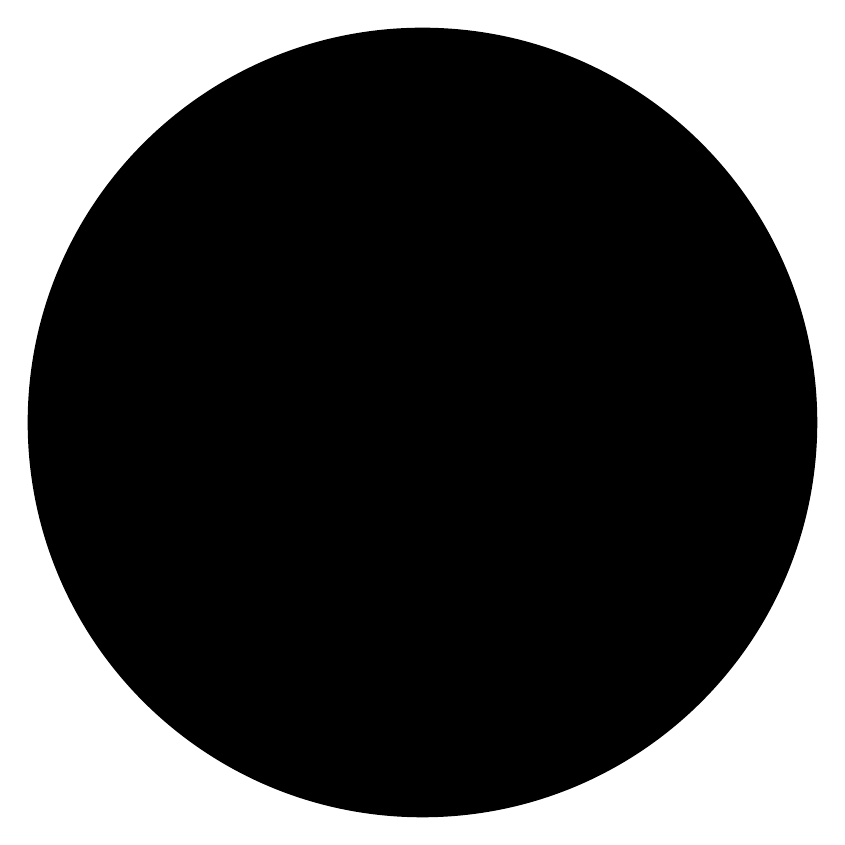
\begin{tikzpicture}
	
	% draw bandgap-guiding fibre, light confined to a low-index region by photonic bandgap with high-index "holes" in the cladding (dark)
	\begin{scope}[shift={(0,0)}]
		%fibre outline
		%\hexagon{\hexSize}{(0,0)}{thick}{\coreFill}
		\filldraw[thick, fill=\coreFill] (0,0) circle (\hexSize);
	
		%fibre cores using loopy loops		
		\foreach \y in {0,2,...,8} {
			\pgfmathsetmacro{\z}{9-0.5*\y}
			\foreach \x in {0,...,\z} {
				\filldraw[fill=\airFill, thick] (\x*\coreSep, \y*\coreSepHeight) circle (\coreSize);
				\filldraw[fill=\airFill, thick] (-\x*\coreSep, \y*\coreSepHeight) circle (\coreSize);
				\filldraw[fill=\airFill, thick] (\x*\coreSep, -\y*\coreSepHeight) circle (\coreSize);
				\filldraw[fill=\airFill, thick] (-\x*\coreSep, -\y*\coreSepHeight) circle (\coreSize);
			}
		}
		\foreach \y in {1,3,...,9} {
			\pgfmathsetmacro{\z}{9-0.5*\y}
			\foreach \x in {0,1,...,\z} {
				\filldraw[fill=\airFill, thick] (\x*\coreSep + 0.5*\coreSep, \y*\coreSepHeight) circle (\coreSize);
				\filldraw[fill=\airFill, thick] (-\x*\coreSep - 0.5*\coreSep, \y*\coreSepHeight) circle (\coreSize);
				\filldraw[fill=\airFill, thick] (\x*\coreSep + 0.5*\coreSep, -\y*\coreSepHeight) circle (\coreSize);
				\filldraw[fill=\airFill, thick] (-\x*\coreSep - 0.5*\coreSep, -\y*\coreSepHeight) circle (\coreSize);
			}
		}
	
		% draw "core" as abscence of periodic pattern
		\filldraw[thick, draw=\airFill, fill=\airFill] (0,0) circle (3*\coreSize);
		\filldraw[thick, draw=\airFill, fill=\airFill] (\coreSep,0) circle (\coreSize);
		\filldraw[thick, draw=\airFill, fill=\airFill] (-\coreSep,0) circle (\coreSize);
		\filldraw[thick, draw=\airFill, fill=\airFill] (0.5*\coreSep,\coreSepHeight) circle (\coreSize);
		\filldraw[thick, draw=\airFill, fill=\airFill] (-0.5*\coreSep,\coreSepHeight) circle (\coreSize);
		\filldraw[thick, draw=\airFill, fill=\airFill] (0.5*\coreSep,-\coreSepHeight) circle (\coreSize);
		\filldraw[thick, draw=\airFill, fill=\airFill] (-0.5*\coreSep,-\coreSepHeight) circle (\coreSize);
	\end{scope}
				
\end{tikzpicture}


\end{document}